\documentclass{beamer}

%\useoutertheme[glossy]{wuerzburg}
\useinnertheme[shadow,outline]{chamfered}
%\usecolortheme{shark}
\usecolortheme{beaver}
\beamertemplatenavigationsymbolsempty

\usefonttheme{professionalfonts}
\let\digamma\relax
\usepackage[scale=0.85,stdmathitalics=true,romanfamily=casual]{lucimatx}
\usefonttheme[stillsansseriftext]{serif}



\usepackage{fancyvrb}

%% Fancy syntax coloring via pygments
\usepackage{minted}
\definecolor{bg}{rgb}{0.95,0.95,0.95}
\usemintedstyle{borland}


\newenvironment{Rcode}
{\VerbatimEnvironment
 \begin{minted}[fontsize=\scriptsize,baselinestretch=1]{r}}%
{\end{minted}}

\newenvironment{Pcode}
{\VerbatimEnvironment
 \begin{minted}[fontsize=\scriptsize,baselinestretch=1]{python}}%
{\end{minted}}

\newenvironment{Code}[1]
{\VerbatimEnvironment
 \begin{minted}[fontsize=\scriptsize,baselinestretch=1]{#1}}%
{\end{minted}}


\usepackage{textfit} % commands \scaletoheight{height}{text} and \scaletowidth{width}{text}

\usepackage{tikz}

\usepackage{tcolorbox}

\newtheorem{Alert}{Alert}
\newtheorem{Highlight}{Highlight}

\newcommand{\Species}[1]{{\rmfamily \itshape #1}}
\newcommand{\Real}{\ensuremath{\mathbb{R}}}
\newcommand{\RealN}{\ensuremath{\mathbb{R}^n}}
\newcommand{\RealP}{\ensuremath{\mathbb{R}^p}}
\newcommand{\Mtx}[1]{\ensuremath{\mathbf{#1}}}
\newcommand{\Inv}[1]{\ensuremath{#1^{-1}}}
\newcommand{\InvMtx}[1]{\ensuremath{\mathbf{#1}^{-1}}}
\newcommand{\Red}[1]{\textcolor{red}{#1}}
\newcommand{\PsInv}[1]{\ensuremath{\mathbf{#1}^{+}}}

\usepackage{booktabs}



% --- Macro \xvec
% From a tex.stackexchange.com answer by Todd Lehman
% http://tex.stackexchange.com/questions/44017/dot-notation-for-derivative-of-a-vector
\makeatletter
\newlength\xvec@height%
\newlength\xvec@depth%
\newlength\xvec@width%
\newcommand{\xvec}[2][]{%
  \ifmmode%
    \settoheight{\xvec@height}{$#2$}%
    \settodepth{\xvec@depth}{$#2$}%
    \settowidth{\xvec@width}{$#2$}%
  \else%
    \settoheight{\xvec@height}{#2}%
    \settodepth{\xvec@depth}{#2}%
    \settowidth{\xvec@width}{#2}%
  \fi%
  \def\xvec@arg{#1}%
  \def\xvec@dd{:}%
  \def\xvec@d{.}%
  \raisebox{.2ex}{\raisebox{\xvec@height}{\rlap{%
    \kern.05em%  (Because left edge of drawing is at .05em)
    \begin{tikzpicture}[scale=1]
    \pgfsetroundcap
    \draw (.05em,0)--(\xvec@width-.05em,0);
    \draw (\xvec@width-.05em,0)--(\xvec@width-.15em, .075em);
    \draw (\xvec@width-.05em,0)--(\xvec@width-.15em,-.075em);
    \ifx\xvec@arg\xvec@d%
      \fill(\xvec@width*.45,.5ex) circle (.5pt);%
    \else\ifx\xvec@arg\xvec@dd%
      \fill(\xvec@width*.30,.5ex) circle (.5pt);%
      \fill(\xvec@width*.65,.5ex) circle (.5pt);%
    \fi\fi%
    \end{tikzpicture}%
  }}}%
  #2%
}
\makeatother

% --- Override \vec with an invocation of \xvec.
\let\stdvec\vec
\renewcommand{\vec}[1]{\xvec[]{#1}}
% --- Define \dvec and \ddvec for dotted and double-dotted vectors.
\newcommand{\dvec}[1]{\xvec[.]{#1}}
\newcommand{\ddvec}[1]{\xvec[:]{#1}}


\usepackage{pifont}
\newcommand{\weblink}{\ding{43}}  % hand with pointing finger

\definecolor{links}{HTML}{2A1B81}
\hypersetup{colorlinks,linkcolor=,urlcolor=magenta}

%\usepackage{amsfonts}
\usepackage{tikz}
\usepackage{caption}
\usepackage{subcaption}

\usepackage[inline]{asymptote}
\usepackage{marvosym} % for male/female symbols




%===========================================================
% Title Info
\title{Scientific Computing for Biologists}
\subtitle{Principal Components Analysis and Eigenanalysis} % (optional)

\author{Instructor: Paul M. Magwene}


\date{24 September 2012}

\begin{document}
%===========================================================
\begin{frame}
\titlepage
\end{frame}

%===========================================================
\begin{frame}
  \frametitle{Overview of Lecture}
  
\begin{itemize}
		\item Principal Components Analysis
		\begin{itemize}
			\item Variable space representation
			\item Subject space representation
			\item Mathematical constrains
			\item PC scores and loadings
			\item Dimension reduction			
		\end{itemize}		
		\item Eigenvectors and eigenvalues	
\end{itemize}

\end{frame}
%===========================================================

%===========================================================
\begin{frame}
  \frametitle{Hands-on Session}
\begin{itemize}
    \item Eigenanalysis and PCA in R
    \item Introduction to Biplots
\end{itemize} 


\end{frame}		
%===========================================================





%===========================================================
\begin{frame}
  \frametitle{General Idea Behind PCA}


\begin{block}{Goal}

Define a new basis for describing your data that has ``nice" properties.

\end{block}
\medskip

By nice we mean:
\begin{itemize}
	\item spans same space as original basis
	\item provides an orthogonal basis
	\item the order of the basis vectors is related to their relative importance
	\item can be used to facilitate low dimensional summaries of high dimensional data
\end{itemize}


\end{frame}

%===========================================================


%===========================================================
\begin{frame}
  \frametitle{Example PC Basis}

\begin{center}
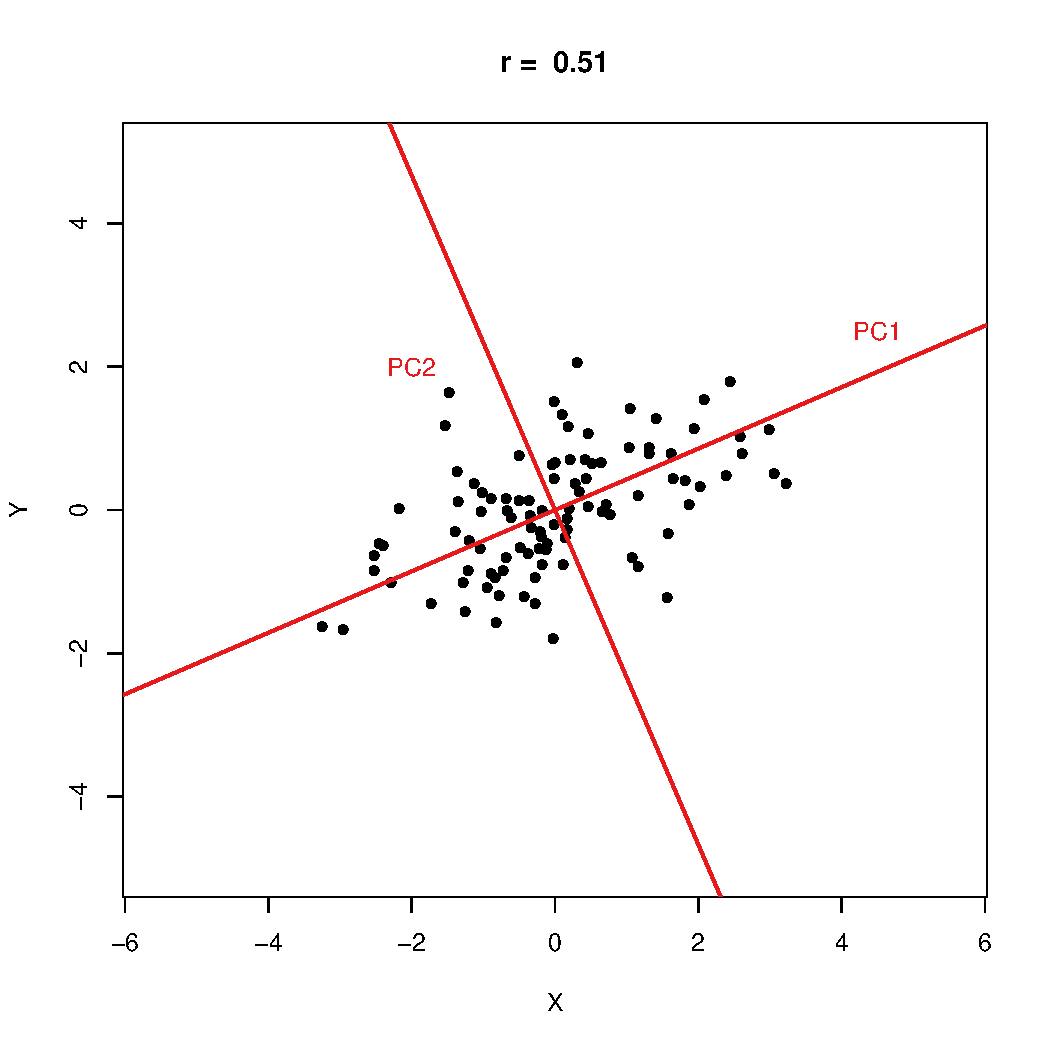
\includegraphics[height=2.75in]{fig-bivariate-pca.pdf}
\smallskip

Variable Space Representation

\end{center}  


\end{frame}
%===========================================================

%===========================================================
\begin{frame}
  \frametitle{Contrast Between PC Axes and Regression}

\begin{center}
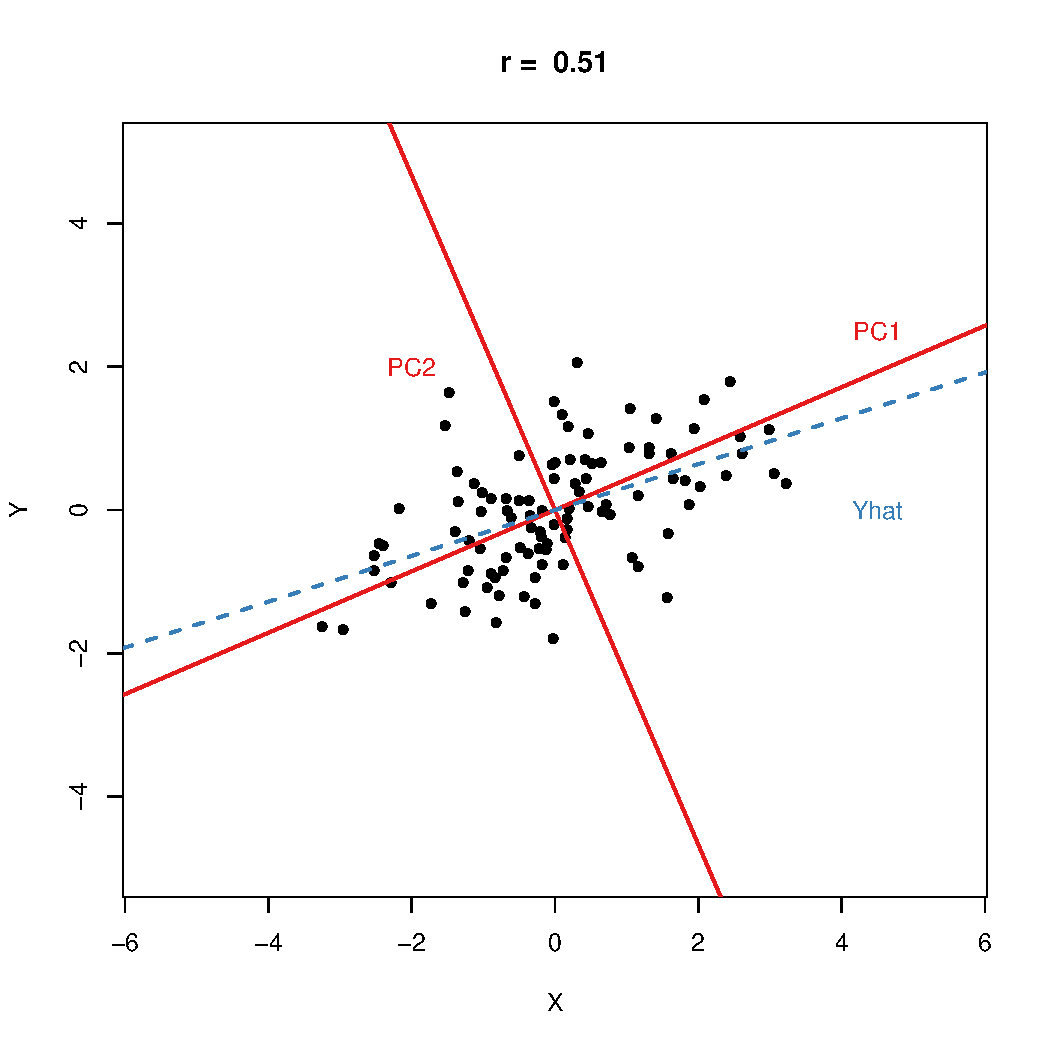
\includegraphics[height=2.75in]{fig-bivariate-pca-wreg.pdf}
\smallskip

\end{center}  

\end{frame}
%===========================================================

%===========================================================
\begin{frame}
  \frametitle{Observations with Respect to the PC Basis}

\begin{center}
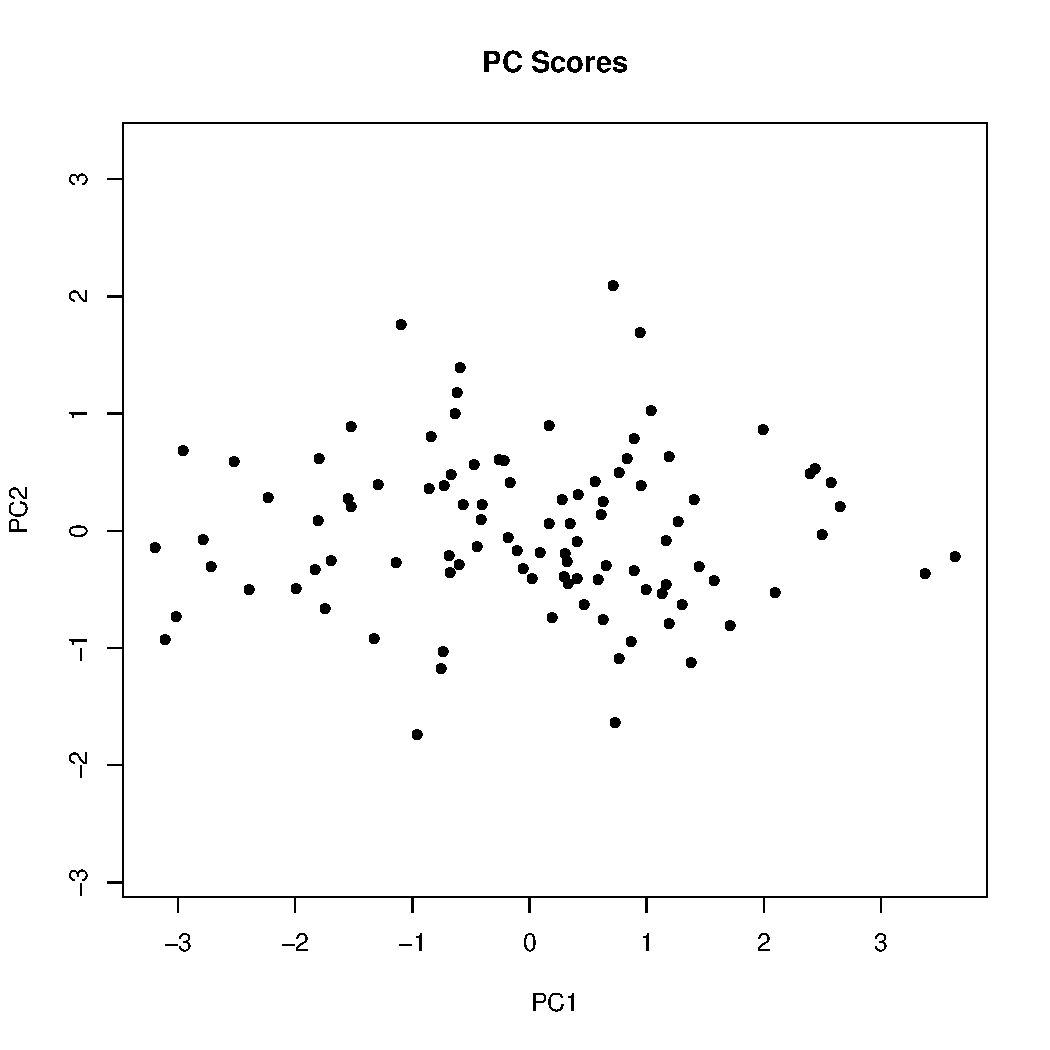
\includegraphics[height=2.75in]{fig-bivariate-pca-scores.pdf}
\smallskip

\end{center}  

\end{frame}
%===========================================================


%===========================================================
\begin{frame}
  \frametitle{Subject Space Representation of PCA}

\begin{center}
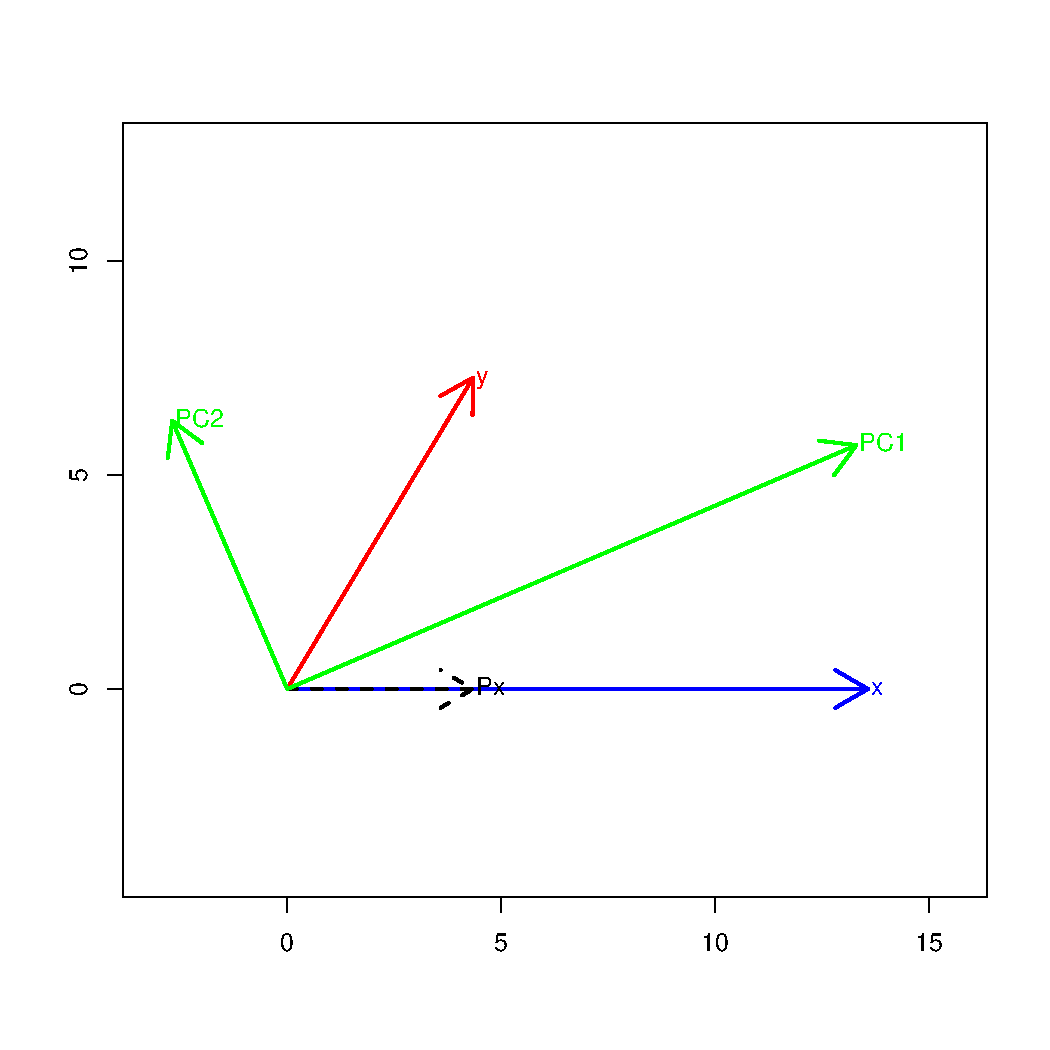
\includegraphics[height=2.5in]{fig-bivariate-pca-vectors.pdf}
\smallskip


\end{center}  

\end{frame}
%===========================================================


%===========================================================
\begin{frame}
  \frametitle{Mathematical Constraints on PCA}

The principal components are linear combinations of the original variables
\medskip

\[ \begin{array}{ccc}
\Mtx{u}_1 & = & a_{11}\Mtx{x}_1 + a_{21}\Mtx{x}_2 + \cdots + a_{p1}\Mtx{x}_p \\
\Mtx{u}_2 & = & a_{12}\Mtx{x}_1 + a_{22}\Mtx{x}_2 + \cdots + a_{p2}\Mtx{x}_p \\
\vdots & & \vdots \\
\Mtx{u}_p & = & a_{1p}\Mtx{x}_1 + a_{2p}\Mtx{x}_2 + \cdots + a_{pp}\Mtx{x}_p \\
\end{array}
\]

\bigskip

\[
\Mtx{U}  =  \left[ \begin{array}{cccc}
\Mtx{u}_1 & \Mtx{u}_2 & \cdots &  \Mtx{u}_p\\
\end{array} \right]
\]

In this formulation the $\Mtx{x}_i$ and $\Mtx{u}_i$ are column vectors.


\end{frame}
%===========================================================

%===========================================================
\begin{frame}
  \frametitle{Mathematical Constraints on PCA, cont.}


\begin{itemize}
	\item The sum of the squared coefficients for each PC is fixed to unity:
\[
a_{1k}^2 + a_{2k}^2 + \cdots + a_{pk}^2 = 1
\]

	\item The sum of the squared lengths for the original variables and the PCs is the same:
\[
|\Mtx{x}_1|^2 + |\Mtx{x}_2|^2 + \cdots + |\Mtx{x}_p|^2 = |\Mtx{u}_1|^2 + |\Mtx{u}_2|^2 + \cdots + |\Mtx{u}_p|^2
\]	

	\item The PCs are orthogonal:
\[
\Mtx{a}_j \cdot \Mtx{a}_k = 0 \mbox{ for all } j \neq k.
\]

	\item The PCs are ordered such that:

\[
 |\Mtx{u}_1|^2 \geq |\Mtx{u}_2|^2  \geq \cdots \geq |\Mtx{u}_p|^2
\]

\end{itemize}

\end{frame}

%===========================================================


%===========================================================
\begin{frame}
  \frametitle{Principal Component Scores}

\begin{block}{Definition}
The PC scores are the components of the original observations with respect to the principal components (i.e. the observations projected into the new basis).
\end{block}
\medskip

If the values of the $i$-th individual in the original variables are:
\[
\begin{array}{cccccc}
\Mtx{r}_i & = & [x_{i1}, & x_{i2}, & \cdots & x_{ip}]
\end{array}
\]

then the score of that individual on the $k$-th principal component axis is given by:

\[
\Mtx{r}_i \cdot \Mtx{a}_k = a_{1k}x_{i1} + a_{2k}x_{i2} + \cdots + a_{pk}x_{ip}
\]

\end{frame}
%===========================================================


%===========================================================
\begin{frame}
  \frametitle{Principal Component Loadings}

The \textbf{loading vector} of the $k$-th PC is:

\[
|\Mtx{u}_k|\Mtx{a}_k
\]

The \textbf{loading} of the $j$-th original variable on the $k$-th PC is:

\[
|\Mtx{u}_k|a_{jk}
\]

\begin{block}{Interpretation}
Loadings give a sense of the relative contribution of each of the original variables to the PCs.
\end{block}

\end{frame}
%===========================================================

%===========================================================
\begin{frame}[fragile]
  \frametitle{Bivariate Example Revisited}

\begin{columns}[c]
  
\column{0.5\textwidth}
\begin{Rcode}
> cov(z)
         [,1]      [,2]
[1,] 1.865551 0.6523660
[2,] 0.652366 0.9248509

> z.pca
Standard deviations:
[1] 1.4830530 0.7687363

Rotation:
            PC1        PC2
[1,] -0.8901780 -0.4556128
[2,] -0.4556128  0.8901780

> A <- z.pca$rotation # coefficients
> L <- diag(z.pca$sdev) # lengths of PCs
> A %*% L  # loadings
          [,1]       [,2]
[1,] -1.320181 -0.3502461
[2,] -0.675698  0.6843122
\end{Rcode}

\column{0.5\textwidth}
\begin{Rcode}
> (A %*% L)**2  # loadings squared
          [,1]      [,2]
[1,] 1.7428784 0.1226723
[2,] 0.4565677 0.4682832
> apply(z, 2, var) # variance of orig.
[1] 1.8655507 0.9248509
\end{Rcode}
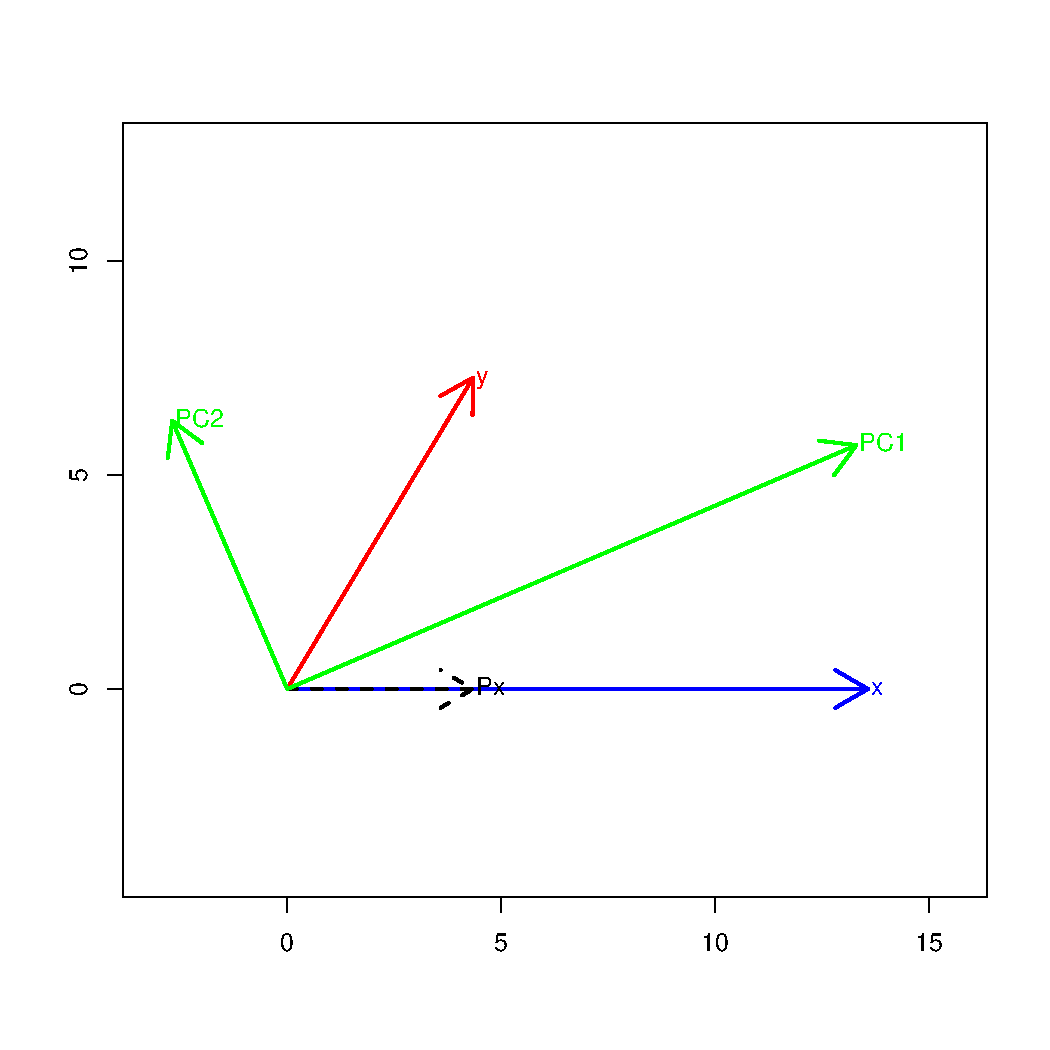
\includegraphics[width=\textwidth]{fig-bivariate-pca-vectors.pdf}

\end{columns}

\end{frame}
%===========================================================



%===========================================================
\begin{frame}
  \frametitle{PCA Cautions and Caveats}

\begin{description}

\item[Scale matters] \mbox{}\\
If the original variables are not measured on comparable scales they should be standardized prior to PCA

\item[PCA emphasizes correlated variables] \mbox{}\\
If one of the original variables is (nearly) independent of the other variables than it will have weak loadings on the major PCs. But this doesn't mean it's unimportant!

\item[PCA does not represent a model] \mbox{}\\
It's simply a transformation of the original data.

\end{description}

\end{frame}

%===========================================================
\begin{frame}
  \frametitle{PCA for Dimension Reduction}


A common application of PCA is to find a lower dimensional representation of a high dimensional data set.
\bigskip 

\begin{block}{Goal}
Capture the majority of the variance with just a few principal component axes.
\end{block}

\end{frame}

%===========================================================

%===========================================================
\begin{frame}
  \frametitle{PCA Example: Jolicoeur and Mosimann's Turtle Data Set}

\begin{itemize}
\item 48 specimens (\Male,\Female), 3 variables (length, width, height)

\item Covariance and correlation matrices:
\footnotesize{
\[
\mathsf{cov}(\Mtx{X}) = \left[ \begin{array}{rrr}
420 & 254 & 165 \\
       & 161 & 102 \\
       &        &   70\\
\end{array}
\right]
\;
;
\;
\mathsf{cor}(\Mtx{X}) = \left[ \begin{array}{ccc}
1 & 0.978 & 0.964 \\
       & 1 & 0.961\\
       &        &   1\\
\end{array}
\right]
\]
} % end \small

\item Principal components (using correlation matrix), proportion of variance:

{\small
\begin{center}
\begin{tabular}{ccc}
PC1 & PC2 & PC3 \\ \hline
0.978 & 0.014 & 0.007
\end{tabular}
\end{center}
} % end \small

\item Principal component loadings:

{\small
\begin{center}
\begin{tabular}{lccc}
&PC1 & PC2 & PC3 \\ \cline{2-4}
L & 0.579 & -0.325 & 0.748 \\
W & 0.578 & -0.483 & -0.657 \\
H & 0.575 & 0.813 & $\sim$0 \\
\end{tabular}
\end{center}
} % end \small



\end{itemize}


\end{frame}

%===========================================================
\begin{frame}
  \frametitle{Turtle PCA Plots}

\begin{center}
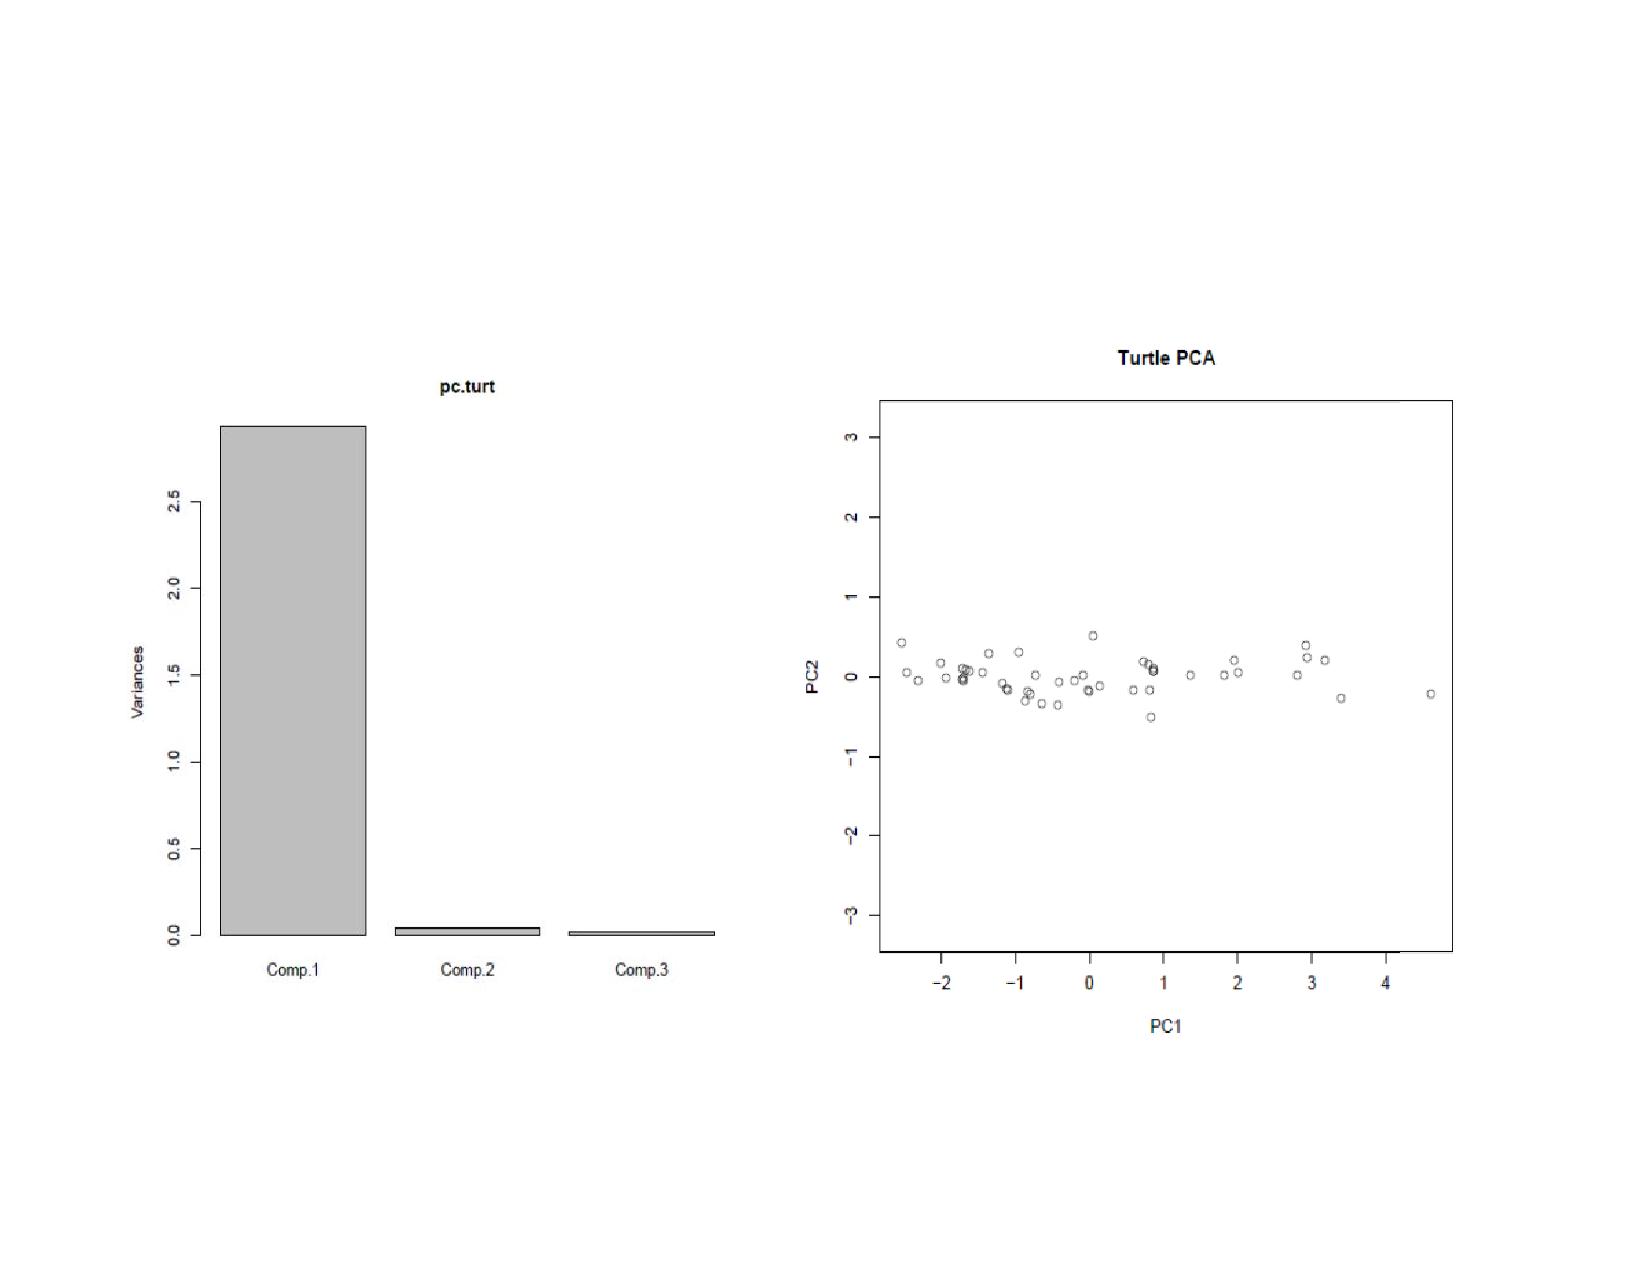
\includegraphics[height=2in]{turtle-pca}
\end{center}
\end{frame}

%===========================================================



%===========================================================
\begin{frame}
  \frametitle{}

\begin{center}
\begin{Huge}
Eigenvectors and Eigenvalues
\end{Huge}
\end{center}
\end{frame}

%===========================================================
\begin{frame}
  \frametitle{Reminder about Linear Transformations}

Recall:

\begin{itemize}
\item Every linear transformation can be represented by a matrix ...

\item ... and conversely, every matrix represents a linear transformation

\item An $n \times p$ matrix represents a transformation from $\RealP$ to $\RealN$.

\item A $p \times p$ matrix is special in that it represent a transformation from $\RealP$ to $\RealP$

\end{itemize}


\end{frame}

%===========================================================
\begin{frame}
  \frametitle{Linear Transformations and Eigenvectors/Eigenvalues}

If $\Mtx{A}$ is a $p \times p$ matrix, then:

\begin{itemize}
\item The \textbf{eigenvectors} of $\Mtx{A}$ represent directions in $\RealP$ that are unchanged by the transformation represented by $\Mtx{A}$

\item Vectors along the directions defined by the eigenvectors may be scaled however. The relative scaling is given by the \textbf{eigenvalues} of $\Mtx{A}$

\end{itemize}
\medskip

if $\Mtx{A}\Mtx{v} = k\Mtx{v}$ for some scalar $k$ than:
\begin{itemize}
\item  $\Mtx{v}$ is an eigenvector of $\Mtx{A}$ 
\item $k$ is it's associated eigenvalue.
\end{itemize}

\end{frame}
%===========================================================
\begin{frame}
  \frametitle{Example Linear Transformation}

\begin{center}
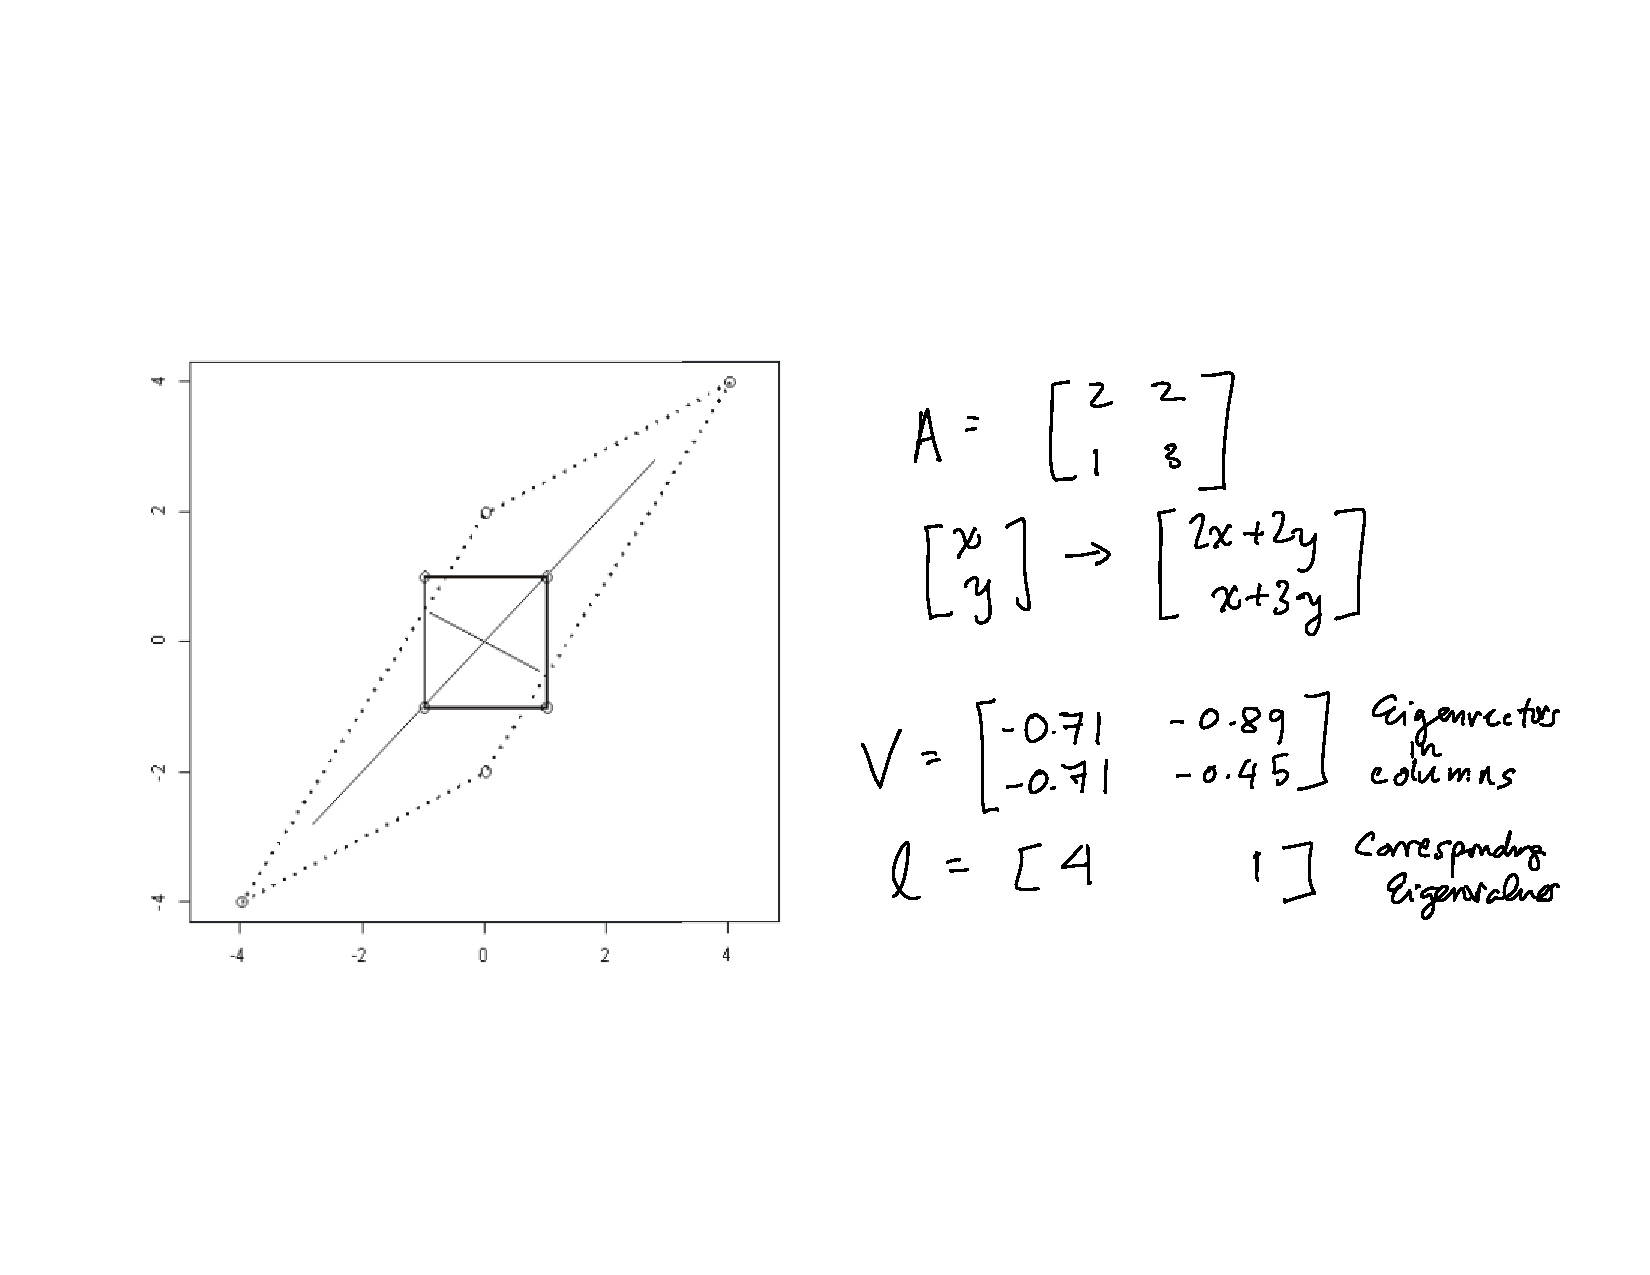
\includegraphics[height=2in]{eigen-example}
\medskip

Note that the eigenvectors above are \emph{not} orthogonal.

\end{center}  

\end{frame}
%===========================================================
\begin{frame}
  \frametitle{More on Eigenvectors and Eigenvalues}

\begin{itemize}
 	\item Eigenvectors/eigenvalues are only defined for square matrices
	\item Eigenvectors are not, in general, orthogonal
\end{itemize}
\smallskip

However, if $\Mtx{A}$ is a real symmetric matrix then:
\begin{itemize}
	\item eigenvectors of $\Mtx{A}$ are guaranteed to be orthogonal
	\item eigenvalues of $\Mtx{A}$ are guaranteed to be real
	\item $\Mtx{A}$ has zero-valued eigenvectors \emph{iff} $\Mtx{A}$ is singular
	\item if $\Mtx{V}$ is the matrix of eigenvectors we can write:
\[
	\Inv{\Mtx{V}} \Mtx{A} \Mtx{V} = \Mtx{D}
\]
where $\Mtx{D}$ is a diagonal matrix with eigenvalues on the diagonal:
\footnotesize{
\[\Mtx{D} = 
 \left[ \begin{array}{rrr}
l_1 &  & 0 \\
       & l_2 & \\
 0      &        &  l_3\\
\end{array}
\right]
\]
} % end \footnotesize

\end{itemize}



\end{frame}
%===========================================================

%===========================================================
\begin{frame}[fragile]
  \frametitle{Calculation of PCs}

Principal components can be calculated by eigenanalysis of the covariance or correlation matrix.
\medskip


\begin{center}
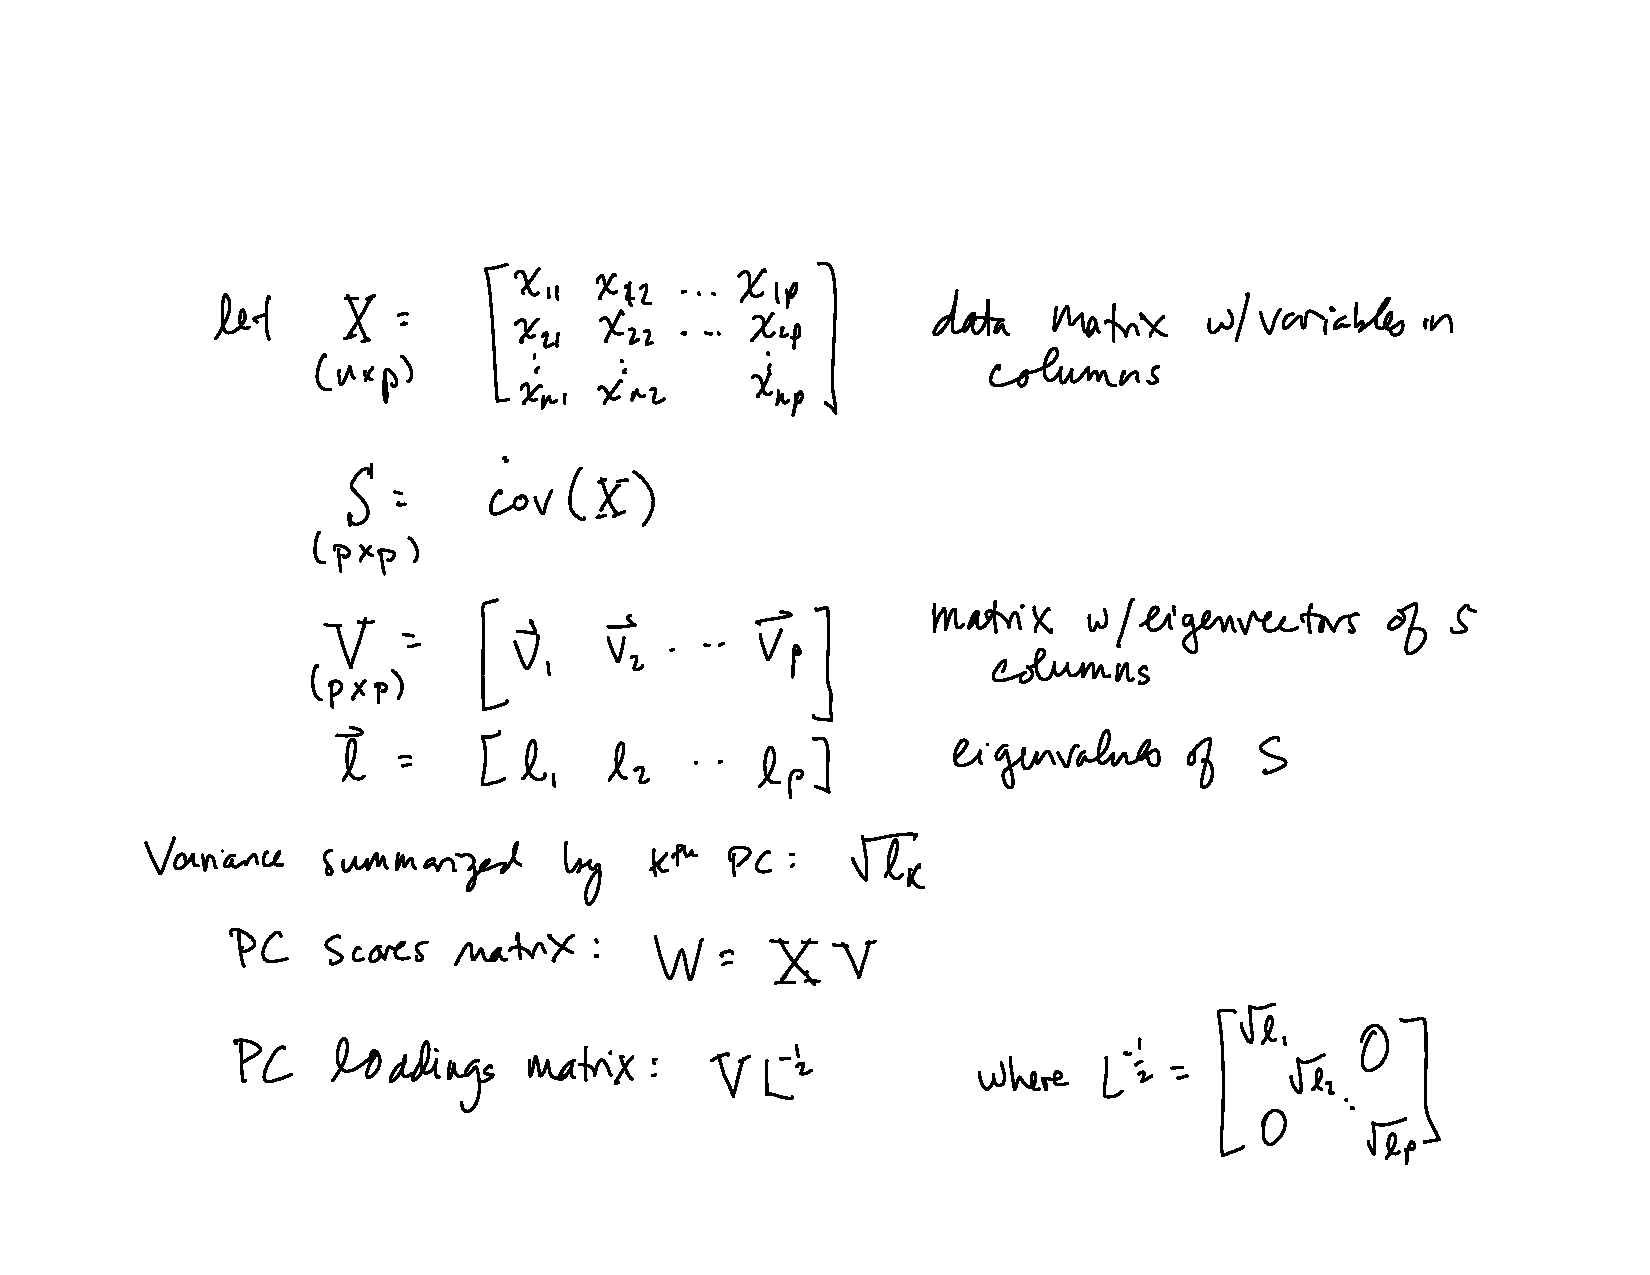
\includegraphics[height=2.7in]{pca-eigen}
\end{center}  


\end{frame}
%===========================================================


\end{document}


%===========================================================
\begin{frame}
  \frametitle{XXX}

\end{frame}
%===========================================================
